\smallskip

 Composition pour dispositif \'electronique en quadriphonie, interpr\'et\'ee le 25/11/16 -- Salle des f\^etes de Perret -- \textit{Kreiz Breizh}.

\bigskip

\noindent \textbf{{\large Pr\'esentation}}
\hrulefill

\bigskip

\texttt{HEX0} est compos\'ee de deux mouvements distincts puisant leurs ressources  dans un panel de partitions \citep{mbb} pr\'eformat\'ees identifi\'ees avec l'extension \textsl{score}. 

\begin{itemize}[leftmargin=0.4in]
\item \textbf{Mouvement I} : \textsc{fractal}. Il s'agit de `fractaliser' dans l'espace une partition de rythmes choisi al\'eatoirement -- ou pas -- parmi le panel pr\'ec\'edemment \'evoqu\'e. L'algorithme est appliqu\'e ind\'ependamment pour chaque phrase dans un rapport de dur\'ee proportionnel.

\item \textbf{Mouvement II} : \textsc{aria}. Airs choisi parmi le panel de partitions traduit par un filtre r\'esonant appliqu\'e \`a une impulsion dans l'espace et une banque de fichiers sons dans un d\'eroulement temporel en termes de grains et de mixage entre les partitions et les samples.
\end{itemize}

\bigskip

\noindent \textbf{{\large Description}}
\hrulefill

\bigskip

  \textbf{\textit{a/ Score }}
  
  \smallskip
  
  \begin{figure}[!hbt]
\begin{center}
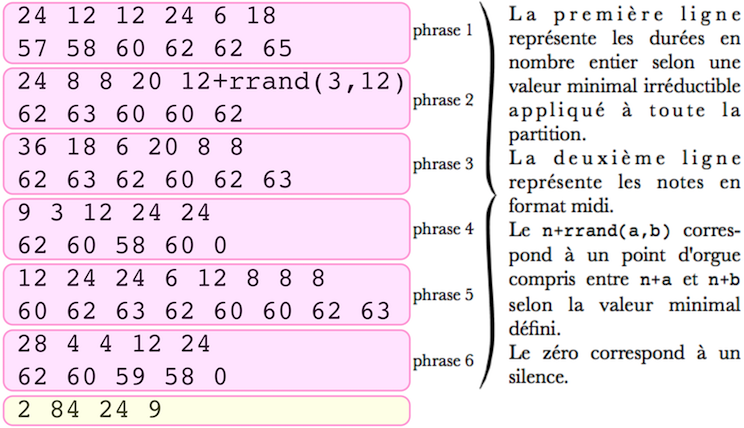
\includegraphics[scale=2.6]{img/4220}
\caption{Description du fichier \textsl{score}. La derni\`ere ligne est r\'eserv\'ee 
au nombre de dimension par \'ev\'enement et par groupe de lignes, et respectivement au tempo + le nombre de valeurs irr\'eductibles associ\'es au tempo + le nombre de r\'ep\'etitions de la partition.}
\label{fig:score}
\end{center}
\end{figure}

  \texttt{HEX0} est conditionn\'e par un corpus  de fichiers partitions permettant de param\'etrer l'ensemble de l'\oe{}uvre. Ces fichiers doivent \^etre formater selon la syntaxe d\'ecrite \`a la figure \ref{fig:score} -- voir aussi \ref{tradscore} page \pageref{tradscore}.
  
%  \clearpage

\bigskip

  \textbf{\textit{b/ } Mixage }
  
  \smallskip
  
  \begin{wrapfigure}{r}{0.45\textwidth}
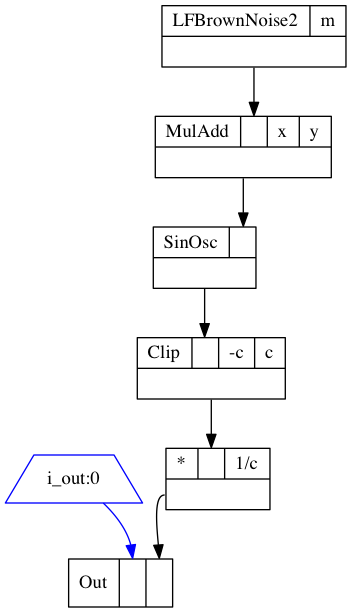
\includegraphics[width=0.9\linewidth]{img/2328} 
\caption{Mixage par modulation de fr\'equence.}
\label{fig:mix}
\end{wrapfigure}

Dans le deuxi\`eme mouvement, le mixage entre le chant et le `grain' est assur\'e par modulation de fr\'equence selon 3 arguments; la dur\'ee minimale $a$ entre 2 \'ev\'enements, la dur\'ee maximale $b$ entre 2 \'ev\'enements et le niveau $c$ d'\'ecr\^etage. 

\smallskip

La modulation de fr\'equence est effectu\'ee sur une onde porteuse sinuso\"idale et une fr\'equence de modulation selon une distribution stochastique lin\'eaire appel\'ee \textit{gendy}\footnote{\textit{Gendy is an implementation of the dynamic stochastic synthesis generator conceived by Iannis Xenakis and described in his book} Formalized Music \citep[chapter 9 pp. 246-254 and chapters 13 and 14 pp. 289-322]{ix}.} avec pour argument la moyenne des dur\'ees -- soit $(a+b)/2$ -- convertie en \textit{hertz} -- soit $m= 2/(a+b)$. 

\smallskip

Cette modulation est ensuite transpos\'ee afin d'osciller selon une fr\'equence d\'efinie par les dur\'ees minimale et maximale pr\'ed\'efinies. Ces dur\'ees sont converti en \textit{hertz} -- soit respectivement $1/a$ et $1/b$. La fr\'equence porteuse doit alors \^etre multipli\'ee par $x=(b+a)/ab$ auquel r\'esultat on ajoute $y=(b-a)/ab$.

\smallskip

L'\'ecr\^etage $c$ permet des paliers de dur\'ee continu pour chaque \'ev\'enement. Celui-ci est normalis\'e en multipliant le r\'esultat par $1/c$ -- voir figure \ref{fig:mixcurve}.

\bigskip

\noindent \textbf{{\large Notes}}
\hrulefill

\bigskip

L'\textsl{UGen} fait parti des \'el\'ements de base permettant la g\'en\'eration et le traitement du signal en termes de computation. L'\textsl{UGen}  \texttt{SplayAz} permet en l'occur- rence de diffuser un signal \`a travers un r\'eseau de canaux audio.

Concernant l'\textsl{UGen} \texttt{SplayAz}, deux arguments optionnels m\'eritent d'\^etre souligner ici : \textsl{spread} et plus particuli\`erement \textsl{center}. Le premier diffuse plus ou moins  quantitativement et respectivement de 1 \`a 0 le signal autour de la valeur du second. Le dernier admet une valeur allant de $-1$ \`a $+1$ traduit par une localisation circulaire impliquant $-1 \Leftrightarrow +1$.
\bigskip

La diff\'erence de configuration des canaux, notamment entre l'\textsl{UGen} \texttt{Pan4}  et l'\textsl{UGen} \texttt{SplayAz}  implique une correction consistant \`a inverser les canaux 2 et 3 avec la m\'ethode \textsl{swap} appliqu\'ee directement sur l'\textsl{UGen} concern\'e, \'etant lui-m\^eme une liste de canaux ordonn\'es.

Par exemple, si l'installation quadriphonique est correct avec l'\textsl{UGen} \texttt{Pan4}, alors la correction se fait sur l'\textsl{UGen} \texttt{SplayAz} de la fa\c con suivante:
 \begin{lstlisting}[basicstyle=\footnotesize\ttfamily,language=Java]
 SplayAz.ar(4, in).swap(2,3)
\end{lstlisting}

\begin{figure}[htbp]
\begin{center}
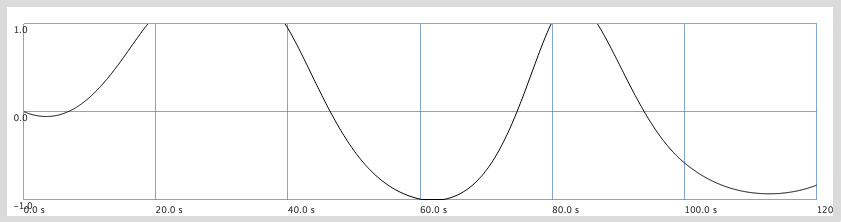
\includegraphics[width=1\linewidth]{img/6890} 
\caption{Mixage oscillant entre 2 signals avec ses plages \'ecr\^et\'ees \`a 0.8 normalis\'ees entre $+1$ et $-1$ sur une dur\'ee de 2 minutes. Le param\'etrage est de 10 secondes pour la dur\'ee minimale et de 30 secondes pour la dur\'ee maximale.}
\label{fig:mixcurve}
\end{center}
\end{figure}